\documentclass[professionalfonts]{beamer}
\usetheme{Copenhagen}

\usepackage{newtxtext,newtxmath}
\usepackage[utf8]{inputenc}
\usepackage[english]{babel}
\usepackage[T1]{fontenc} 
\usepackage{graphicx} 
\usepackage{bibentry} 
\usepackage{array}
\usepackage{tabularx}
\usepackage{tcolorbox}
\usepackage{booktabs}

\usepackage{fontawesome}
\usepackage{bbding} % checkmarks
\usepackage[dvipsnames]{xcolor}

\usepackage{pgfpages}
%\setbeameroption{hide notes} % Only slides
%\setbeameroption{show only notes} % Only notes
%\setbeameroption{show notes on second screen=right} % Both
%\setbeamertemplate{note page}{\pagecolor{yellow!5}\insertnote}
\usepackage{palatino}

% Remove os símbolos de navegação
\usenavigationsymbolstemplate{}

% Cria a cor de padrão da marca (azul, laranja, branco e preto)
\definecolor{UniBlue}{cmyk}{100,90,0,0}
\definecolor{UniOrange}{cmyk}{0,50,100,0}


\addtobeamertemplate{frametitle}{\vspace*{1\baselineskip}}{}

\setbeamerfont{normal text}{size=\fontsize{10pt}{8pt}}
\setbeamerfont{enumerate}{size=\fontsize{10pt}{8pt}}
\setbeamerfont{itemize}{size=\fontsize{10pt}{8pt}}
\setbeamerfont{section in toc}{size=\fontsize{10pt}{8pt}}
\setbeamerfont{subsection in toc}{size=\fontsize{8pt}{8pt}}

\usefonttheme[onlymath]{serif}

% Dados
\title[BPR for MLTC using SVI]{Bayesian Profile Regression for Multimorbidity Clustering at Population Scale}
\author{Dr Jim Rafferty}
\institute{\\[10mm] Swansea University Medical School}
%\date{\\[10mm] March 16, 2022}
\date{}

\usepackage{tikz}
\usetikzlibrary{shapes.geometric, positioning, arrows}
\tikzstyle{start} = [
    rectangle, 
    rounded corners, 
    minimum width=3cm, 
    minimum height=1cm,
    text centered, 
    draw=black, 
    fill=red!30
    ]
\tikzstyle{stop} = [
    rectangle, 
    rounded corners, 
    minimum width=3cm, 
    minimum height=1cm,
    text centered, 
    draw=black, 
    fill=green!30
]
\tikzstyle{process} = [
    rectangle, 
    minimum width=3cm, 
    minimum height=1cm, 
    text centered, 
    draw=black, 
    fill=orange!30
]
\tikzstyle{arrow} = [thick,->,>=stealth]

\newcommand*\oldmacro{}%
\let\oldmacro\insertshorttitle%
\renewcommand*\insertshorttitle{%
  \oldmacro\hfill%
  \insertframenumber\,/\,\inserttotalframenumber}

\begin{document}

\def\beamer@andinst{\\[5em]}
\frame{\titlepage}




\section{Introduction}

\begin{frame}{Acknowledgements}

\begin{center}
    Reference: \url{https://arxiv.org/abs/2602.24038}
    
    \vspace{1em}
    
    \begin{tabular}{cccc}
         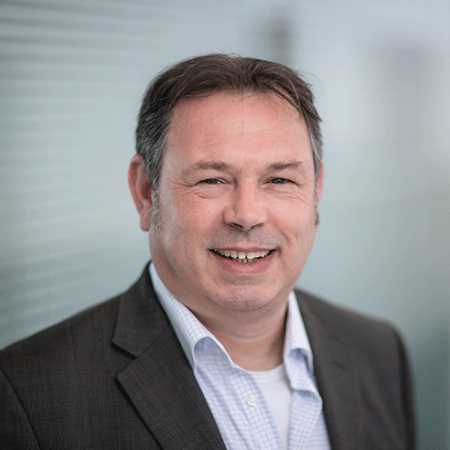
\includegraphics[height=5em]{Keith-Abrams.png} &
         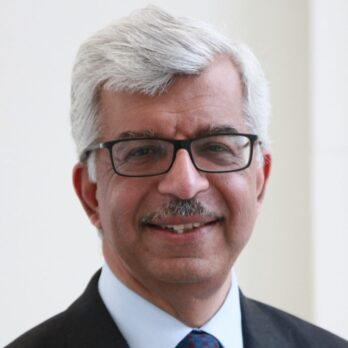
\includegraphics[height=5em]{munir.jpg} & 
         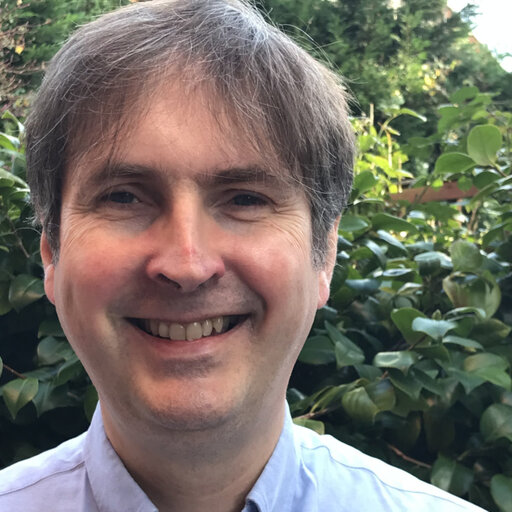
\includegraphics[height=5em]{Mark-Davies.jpg} &
         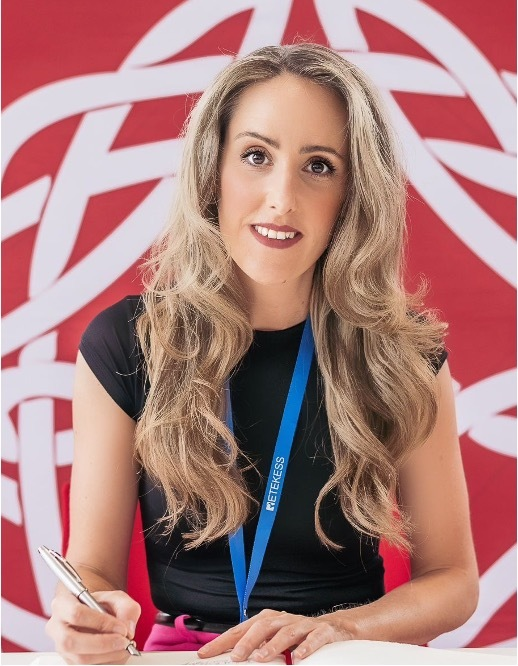
\includegraphics[height=5em]{RKO_Headshot_2025.jpg}
    \end{tabular}
    
    \vspace{1em}
    
    
\includegraphics[height=3em]{HDRUK.jpg}
\end{center}
    
\end{frame}

\begin{frame}{Project aims}

\begin{itemize}
    \item Find clusters of MLTC in EHRs held in SAIL
    \item Write a BPR model that can be fit using SVI 
    \item Validate model performace using simulation studies
\end{itemize}
    
\end{frame}

\section{Bayesian Profile Regression}

\begin{frame}{Bayesian Profile Regression}

    \begin{flushright}
        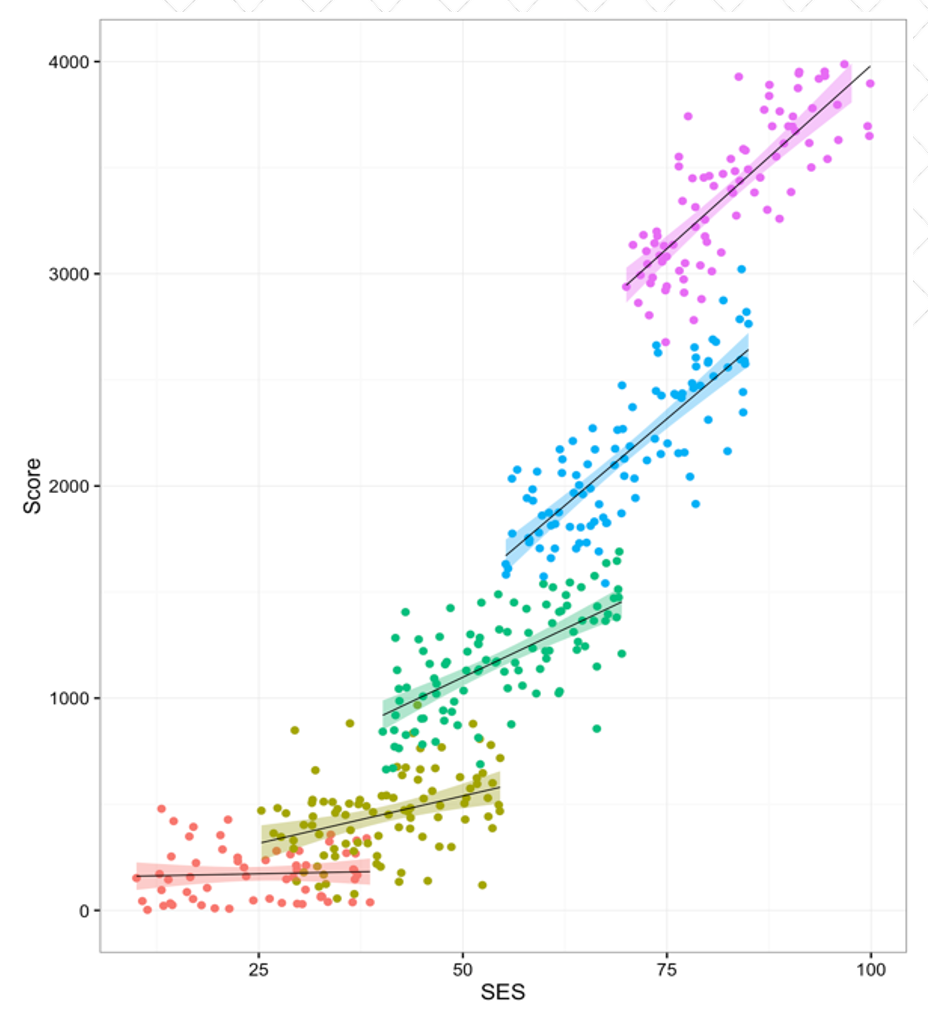
\includegraphics[height=14em]{BPR-ed_ses.png}
        \scalebox{0.3}{Image taken from \url{https://www.r-bloggers.com/2016/10/multilevel-modeling-of-educational-data-using-r-part-1/} accessed 17th April 2026}
        \end{flushright}
\end{frame}

\begin{frame}{Bayesian Profile Regression}

    \begin{flushright}
        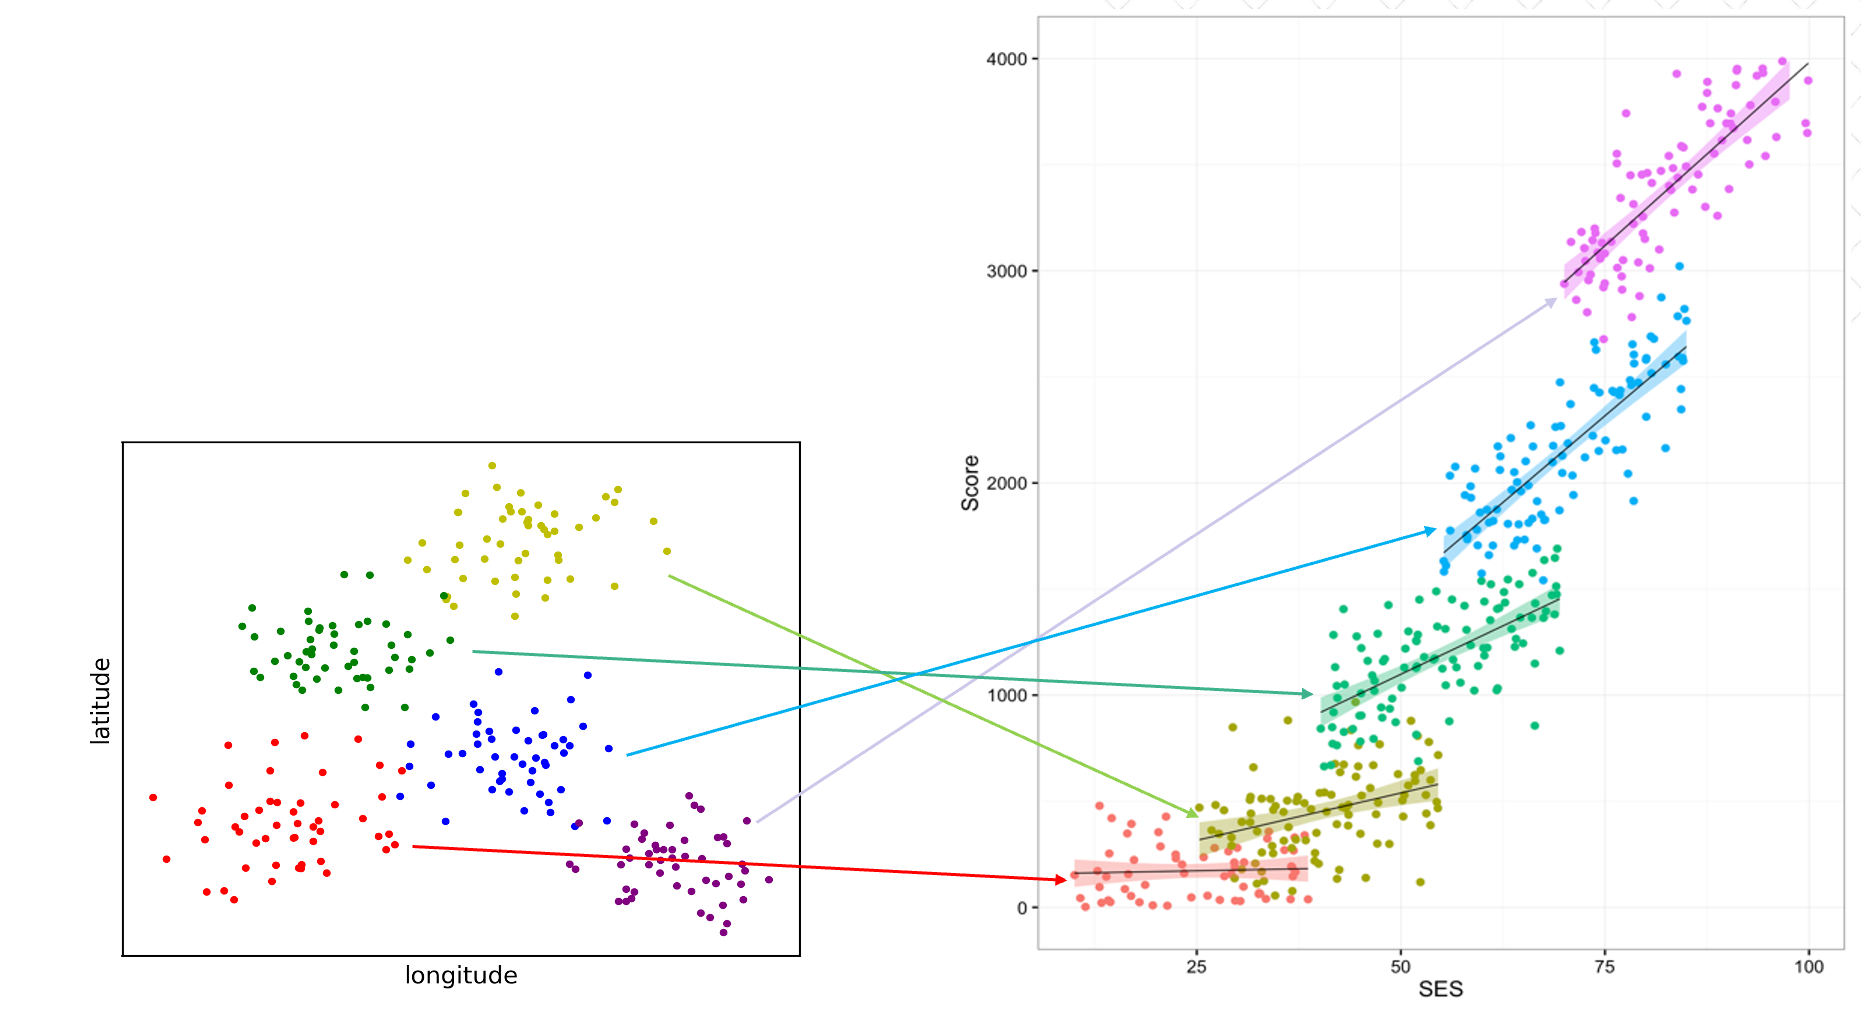
\includegraphics[height=14em]{BPR-ed_ses_full.png}
        \scalebox{0.3}{Image taken from \url{https://www.r-bloggers.com/2016/10/multilevel-modeling-of-educational-data-using-r-part-1/} accessed 17th April 2026}
    \end{flushright}
    
\end{frame}

\begin{frame}{Aside - Dirichlet Process Mixture models}
    \begin{center}
        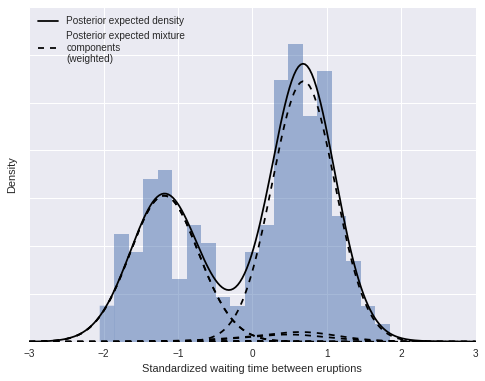
\includegraphics[width=0.6\columnwidth]{DPMM_old_faithful.png}    
    \end{center}
    \begin{flushright}
        \scalebox{0.3}{Image taken from \url{https://austinrochford.com/posts/2016-02-25-density-estimation-dpm.html} accessed 17th April 2026}    
    \end{flushright}
\end{frame}

\begin{frame}{Bayesian Profile Regression}
    \begin{flushright}
        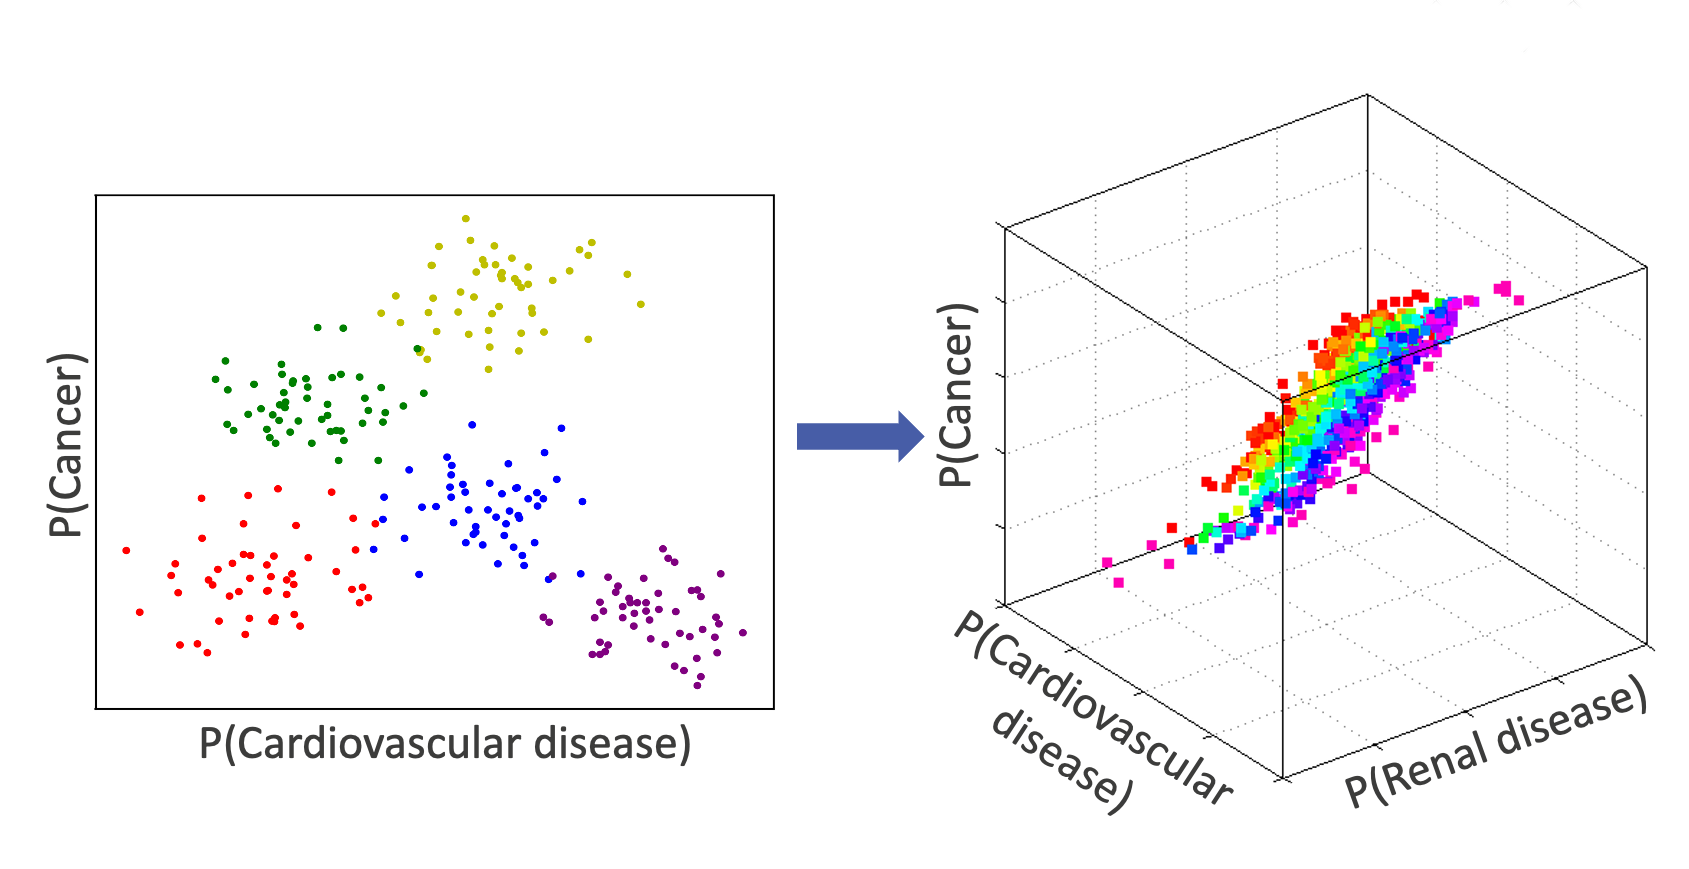
\includegraphics[height=14em]{BPR-MLTC.png}
        \scalebox{0.3}{Image courtesy of Rhiannon Owen}
    \end{flushright}
\end{frame}

\begin{frame}{References}
\begin{itemize}
    \item Molitor J et al. Bayesian profile regression with an application to the National Survey of Children's Health. Biostatistics. 2010 Jul 1;11(3):484-98.
    \item Liverani S et al. PReMiuM: An R package for profile regression mixture models using Dirichlet processes. Journal of statistical software. 2015 Mar 20;64:1-30.
\end{itemize}
    
\end{frame}

\section{Stochastic Variational Inference}

\begin{frame}{Standard fitting methods}
    \begin{itemize}
        \item In a Bayesian framework we calculate the full posterior distribution rather than just point estimates
        \item Normally done with MCMC sampling.
        \item MCMC is computationally quite expensive.
    \end{itemize}
\end{frame}


\begin{frame}{Stochastic Variational Inference}
\pause
\begin{center}
    
    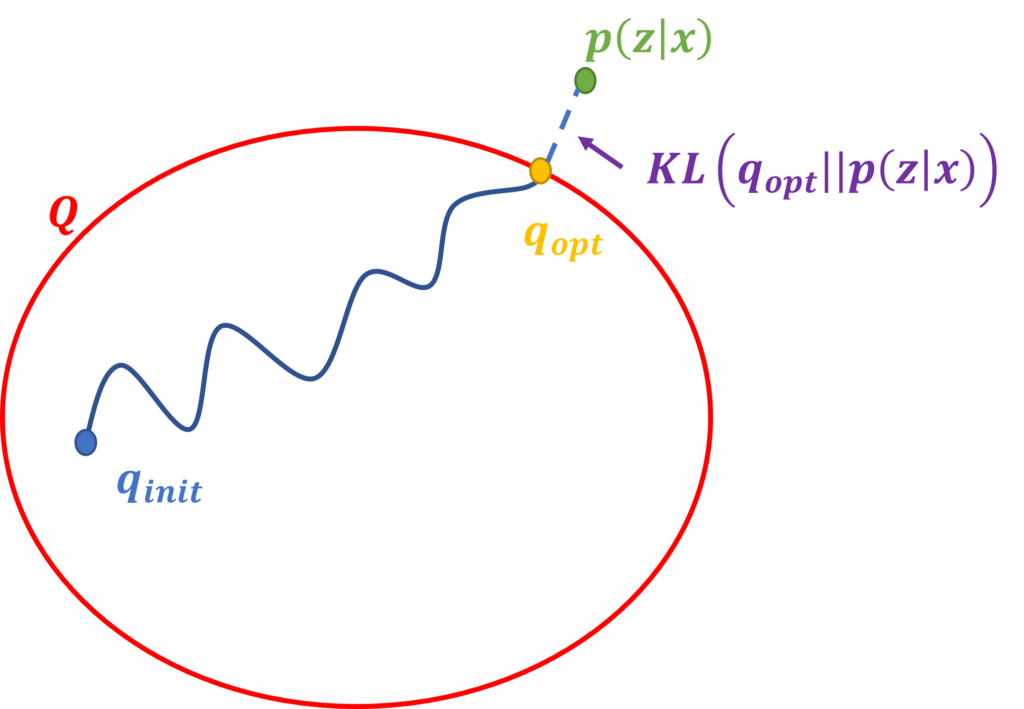
\includegraphics[width=0.6\columnwidth]{SVI.png}\\
    
\end{center}
    \begin{flushright}
        \scalebox{0.4}{from \url{https://meerkatstatistics.com/courses/variational-inference-in-r/} accessed 17th April 2026}
    \end{flushright}
    
\end{frame}



\begin{frame}{Advantages \& Disadvantages}

\begin{center}
    \begin{tabular}{c|c}
        No-U-Turn Sampler & Stochastic Variational Inference \\
        \hline
        {\color{ForestGreen}\CheckmarkBold} Convergence guarantees & {\color{red} \XSolidBrush} No convergence guarantees \\
        {\color{ForestGreen}\CheckmarkBold} Convergence diagnostics & {\color{yellow} \textbf{-}} Convergence diagnostics\\
        %{\color{ForestGreen}\CheckmarkBold} No choice needed & {\color{yellow} \textbf{-}} Choice\\
        {\color{red} \XSolidBrush \XSolidBrush}  Computationally expensive & {\color{ForestGreen}\CheckmarkBold \CheckmarkBold} Computationally efficient 
    \end{tabular}    
\end{center}

    
\end{frame}


\section{Results \& Future work}


\begin{frame}{Results - Simulation study}
    \begin{center}
        \begin{tabular}{cc}
             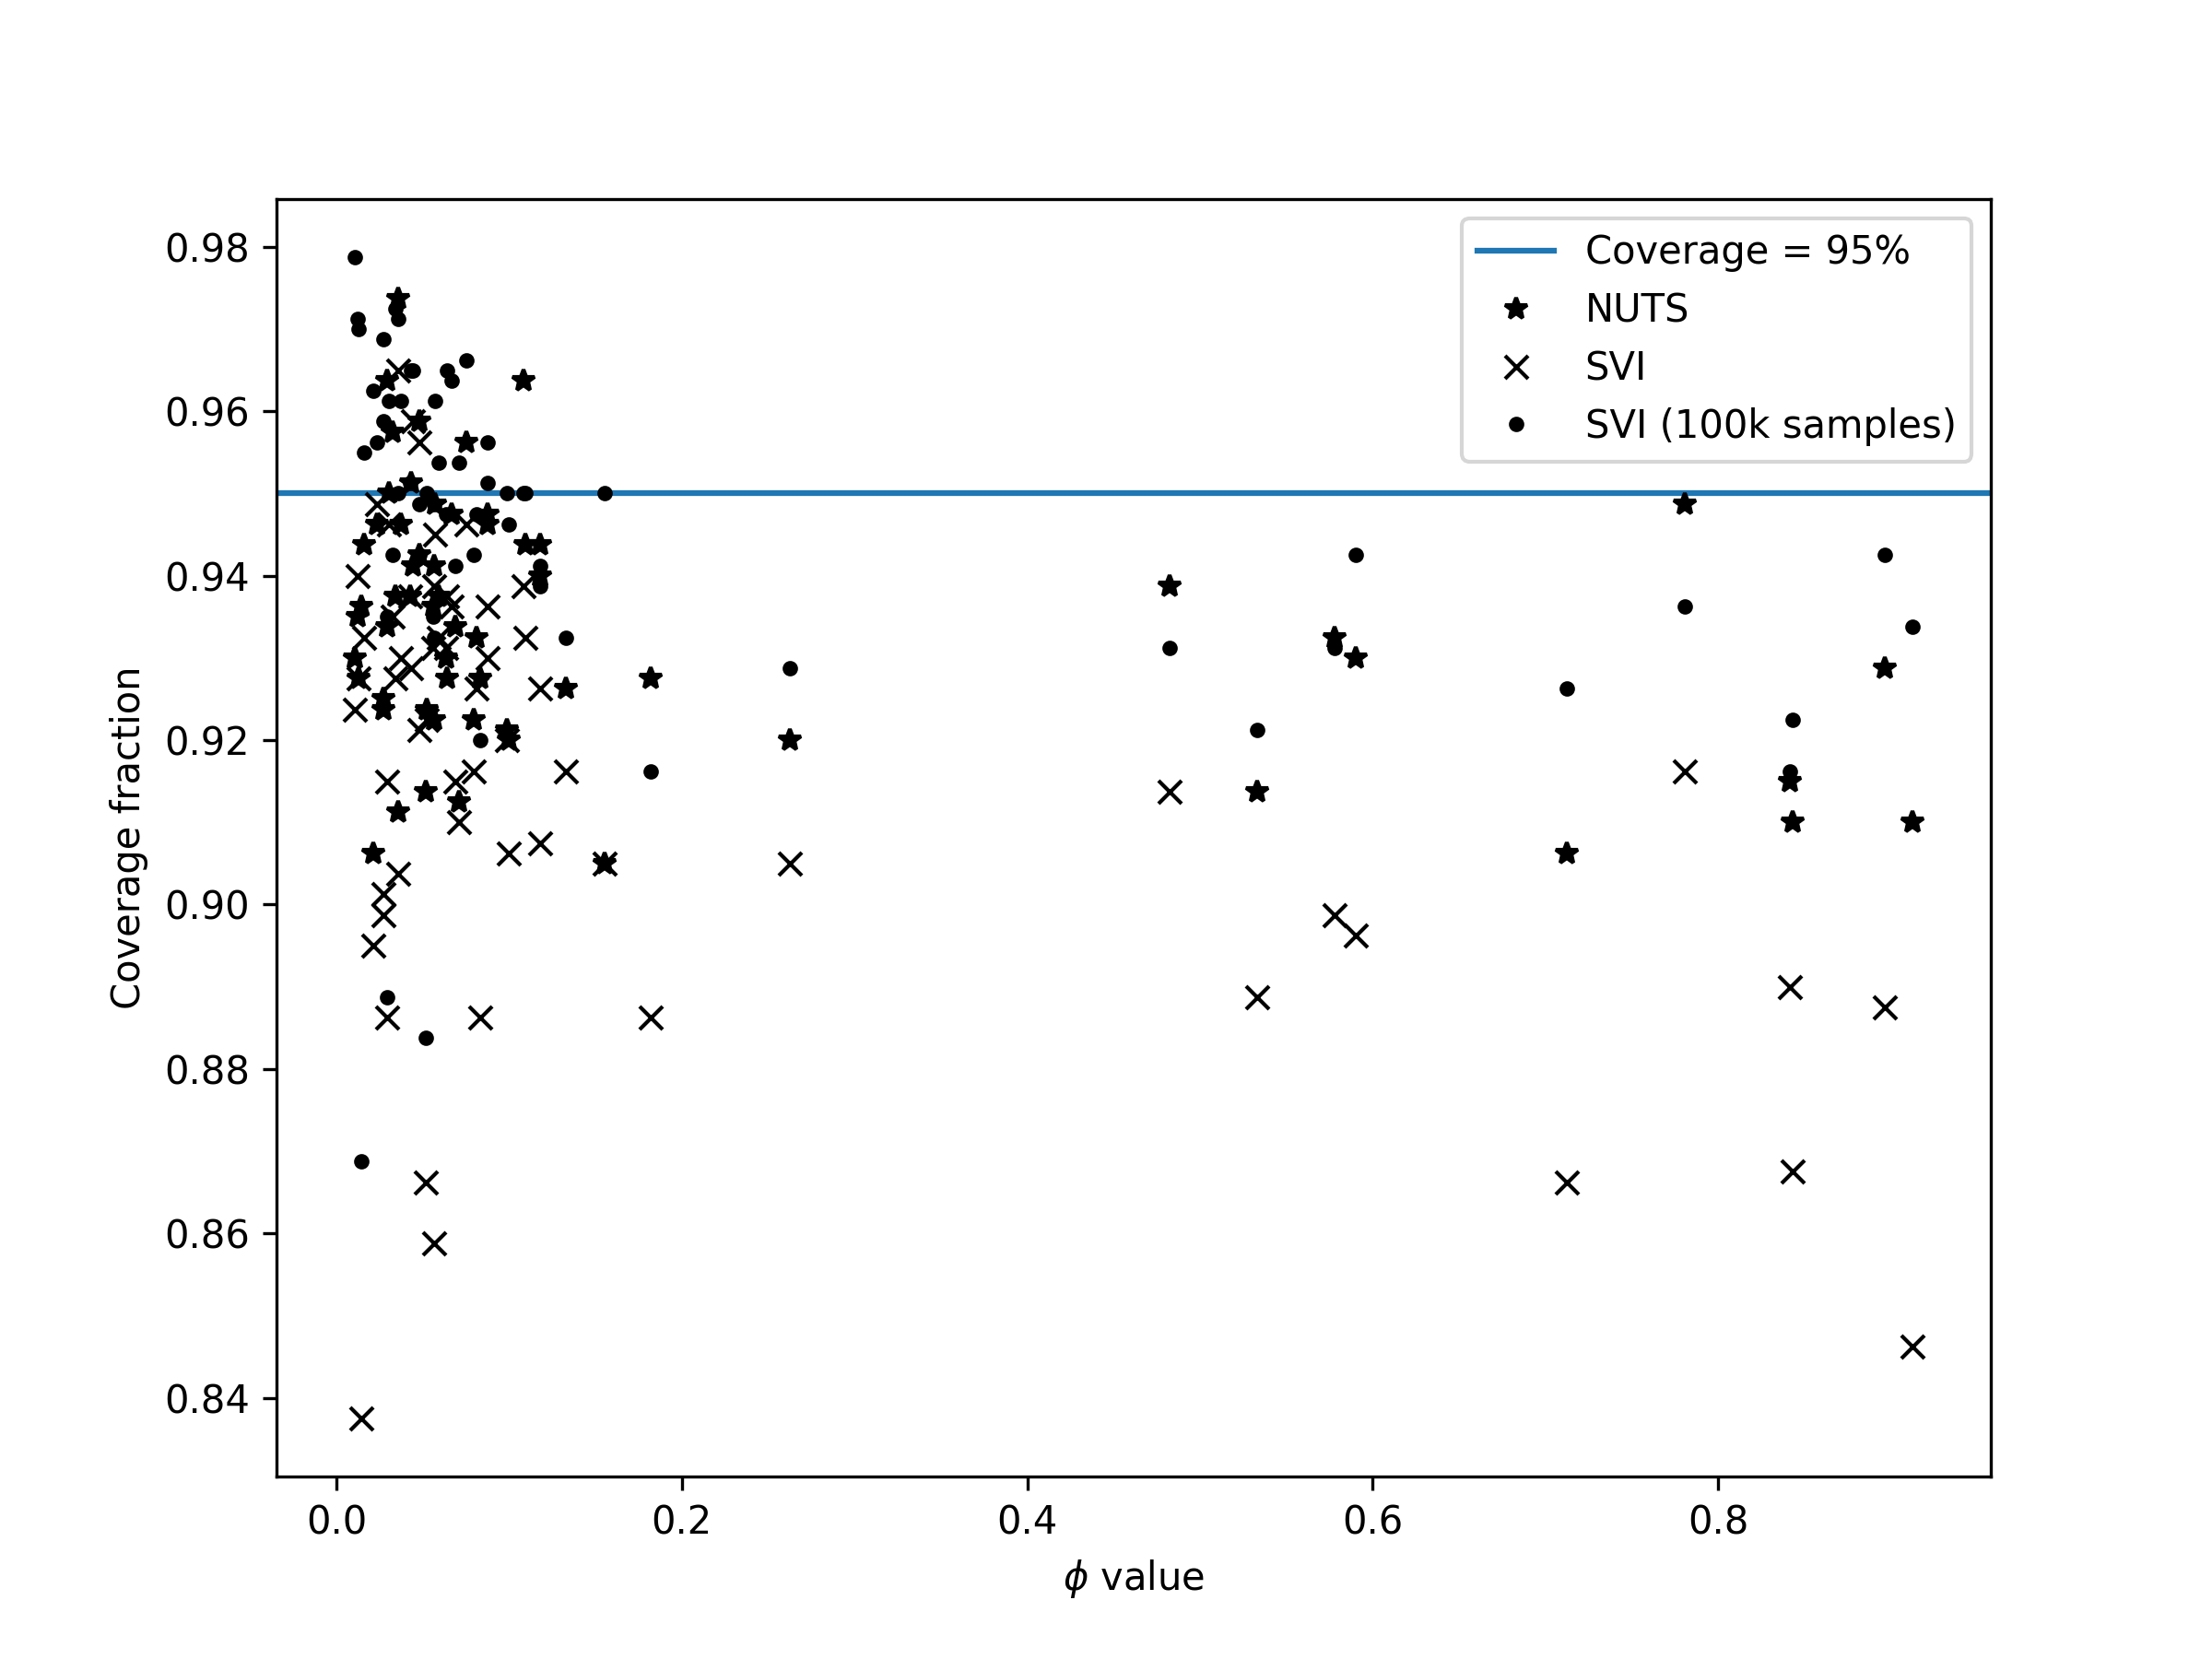
\includegraphics[width=0.45\columnwidth]{phi_coverage.png}&  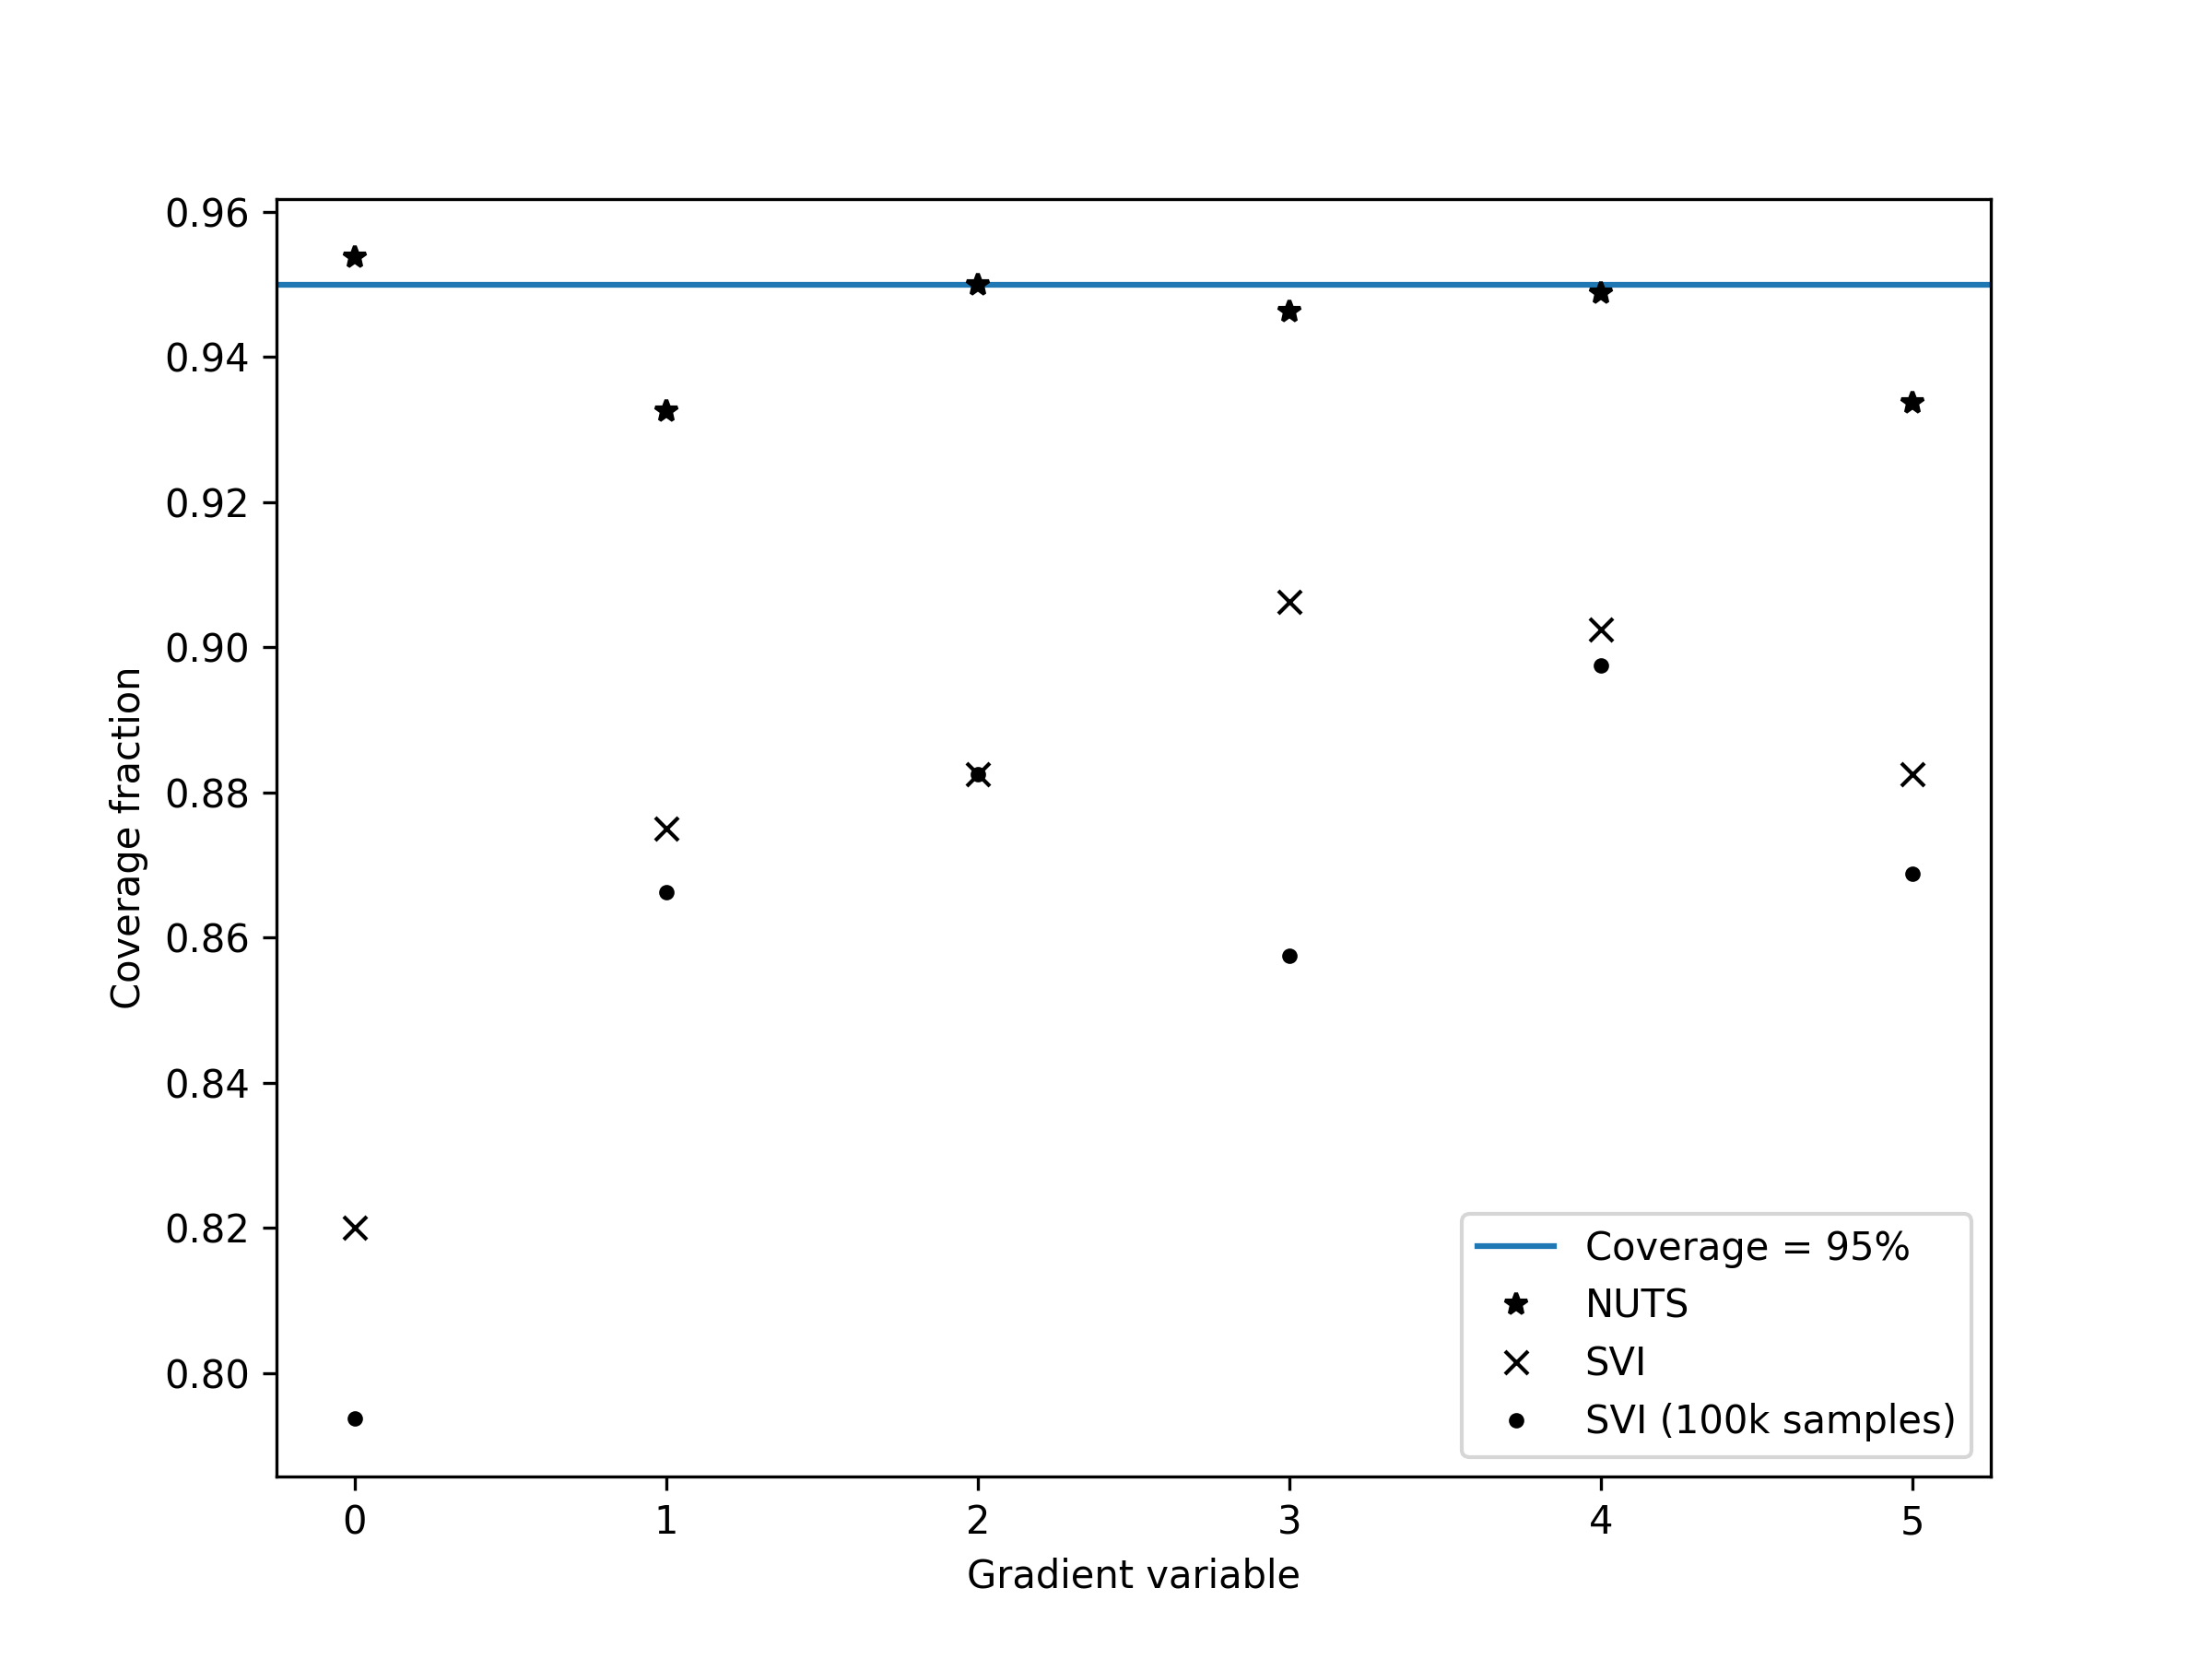
\includegraphics[width=0.45\columnwidth]{gradient_coverage.png}
        \end{tabular}
    \end{center}
\end{frame}



\begin{frame}{Results - SAIL analysis}

    \begin{center}

        \begin{tabular}{m{0.4\columnwidth}m{0.6\columnwidth}}
            {\tiny  
            \begin{tabular}{ll}
                \toprule
              Variable &  N(\%) / Mean(SD)\\
              \midrule
              Population N & 1296463 \\
              Male Sex N(\%) & 631453 (48.70\%)\\
              Age Mean (SD) (years) & 42.51 (15.95) \\
              Died N(\%) & 160709 (12.40\%) \\
              Total Follow up (years) & 20949059\\
              \bottomrule
            \end{tabular}
            } 
             &  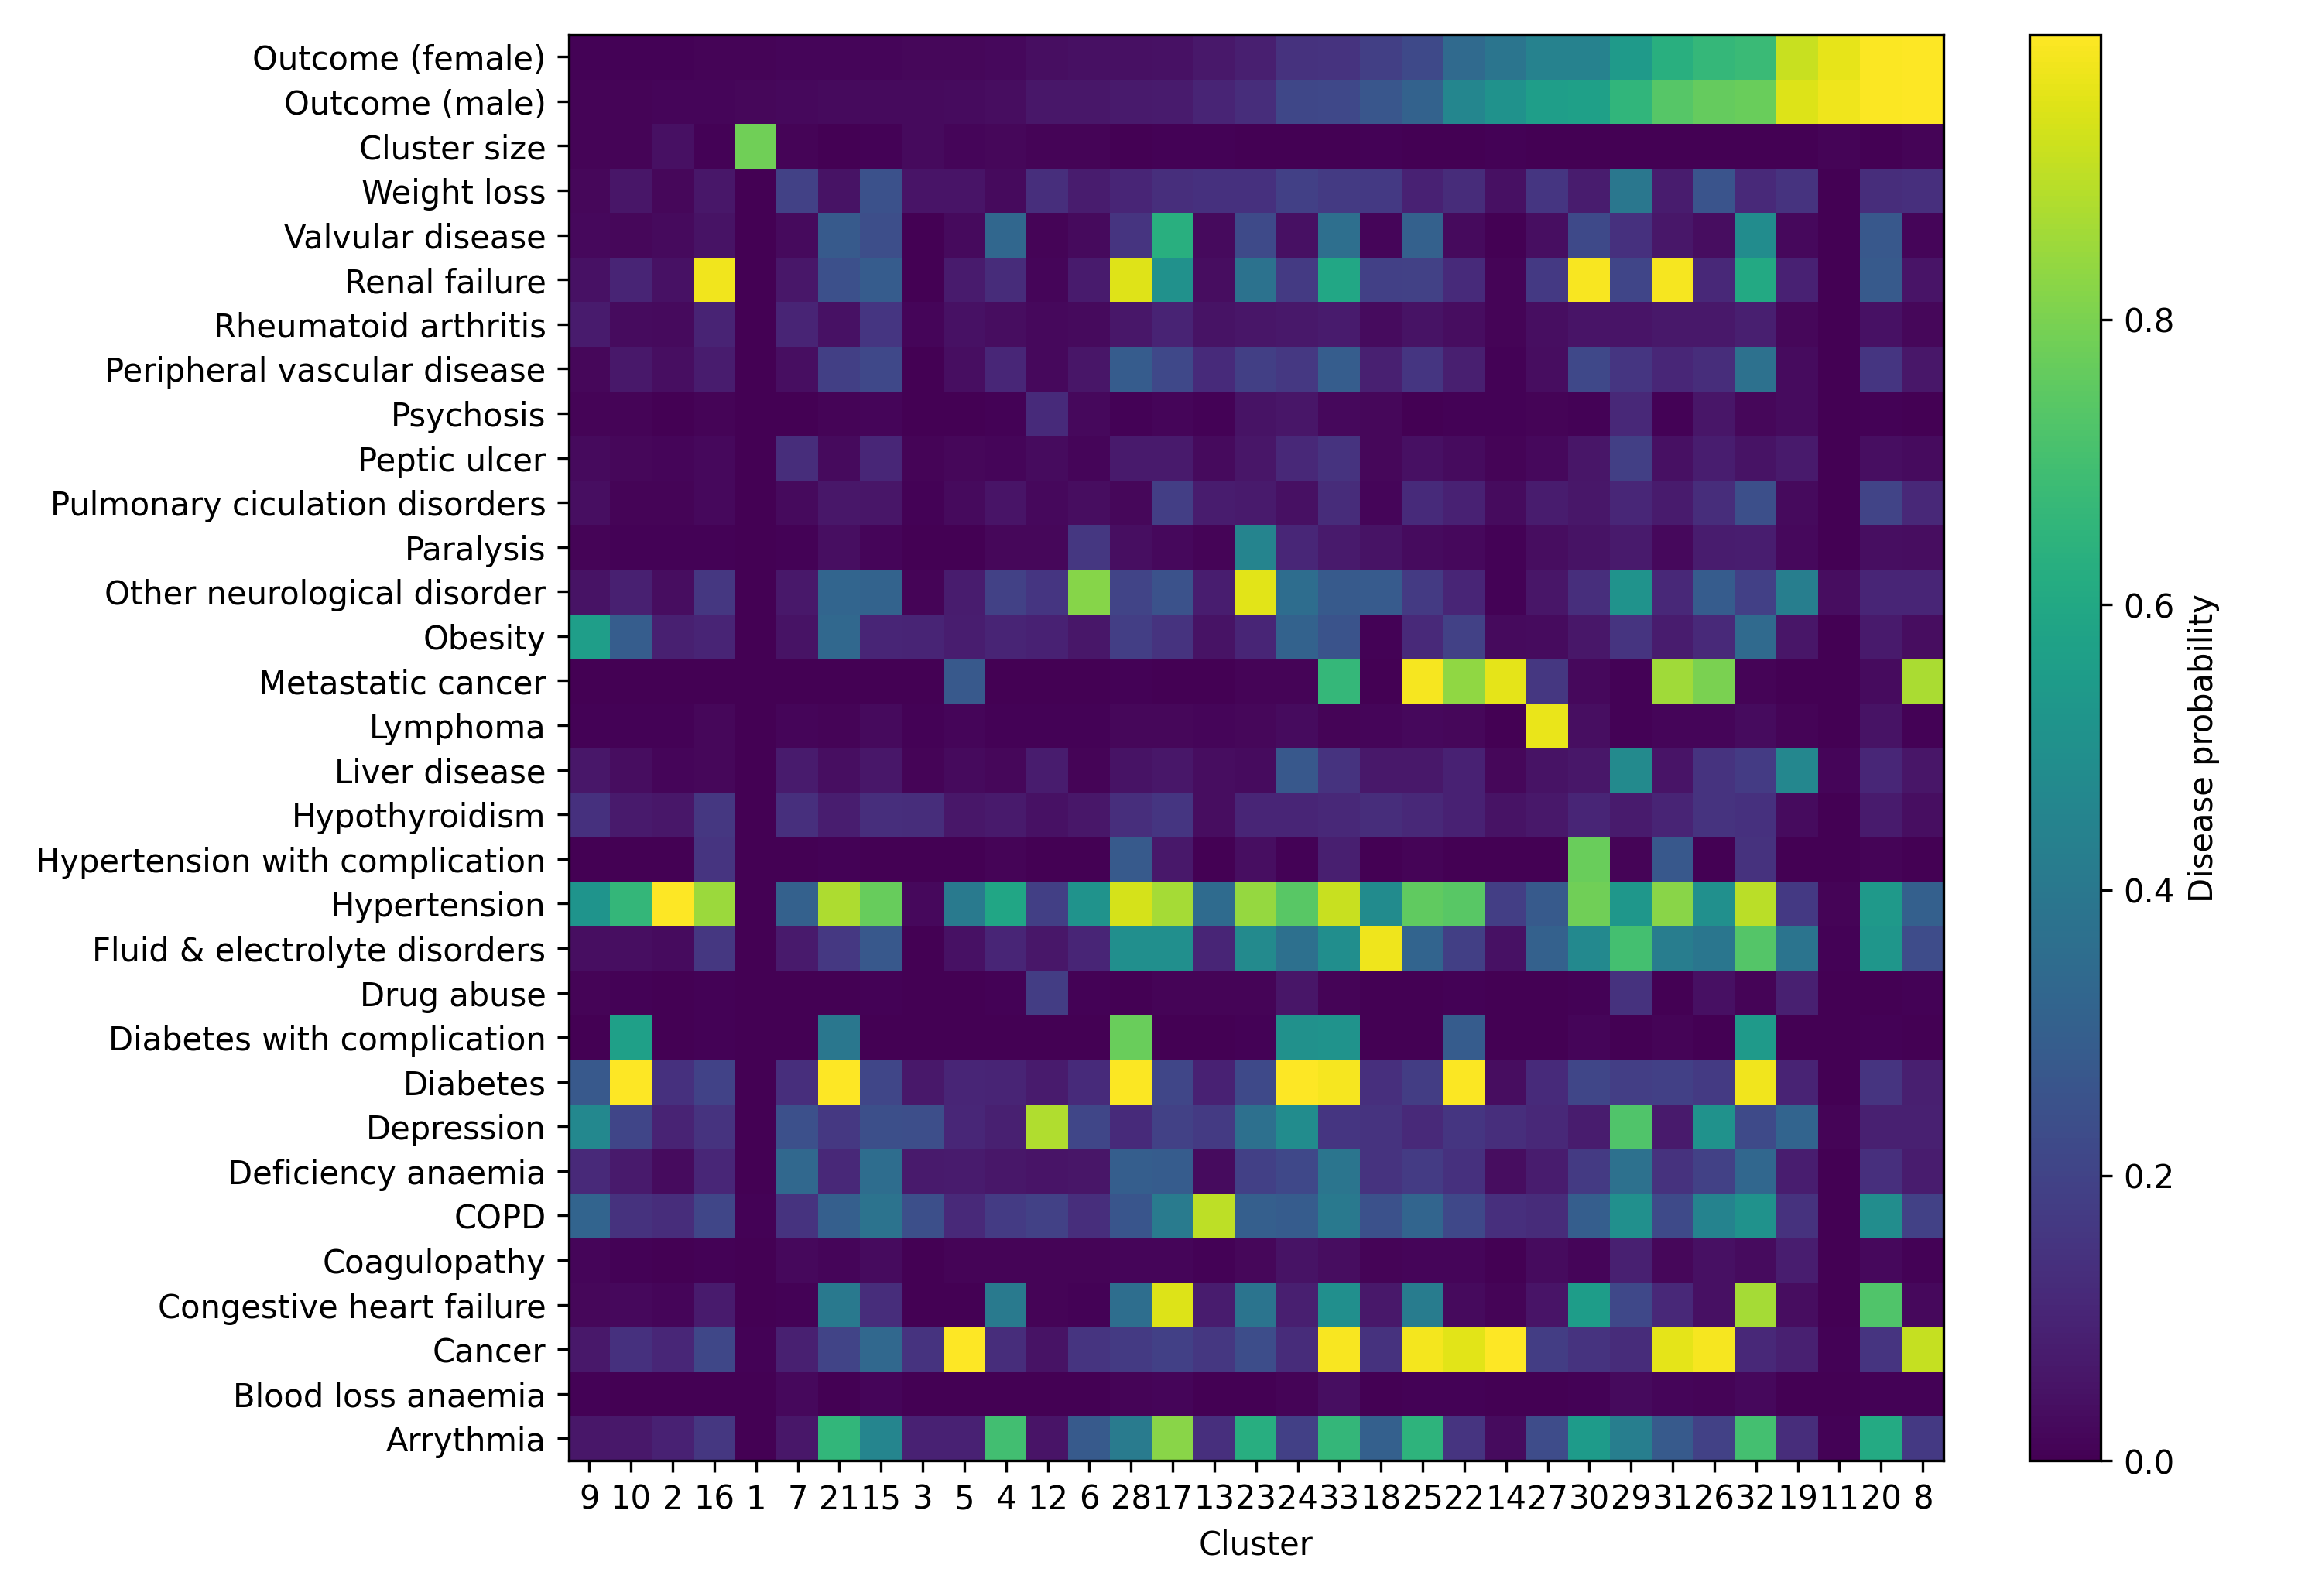
\includegraphics[width=0.6\columnwidth]{SAIL_probability_heatmap_linscale.png}
        \end{tabular}
    \end{center}
        
\end{frame}

\begin{frame}{Results - SAIL analysis}

\begin{center}
    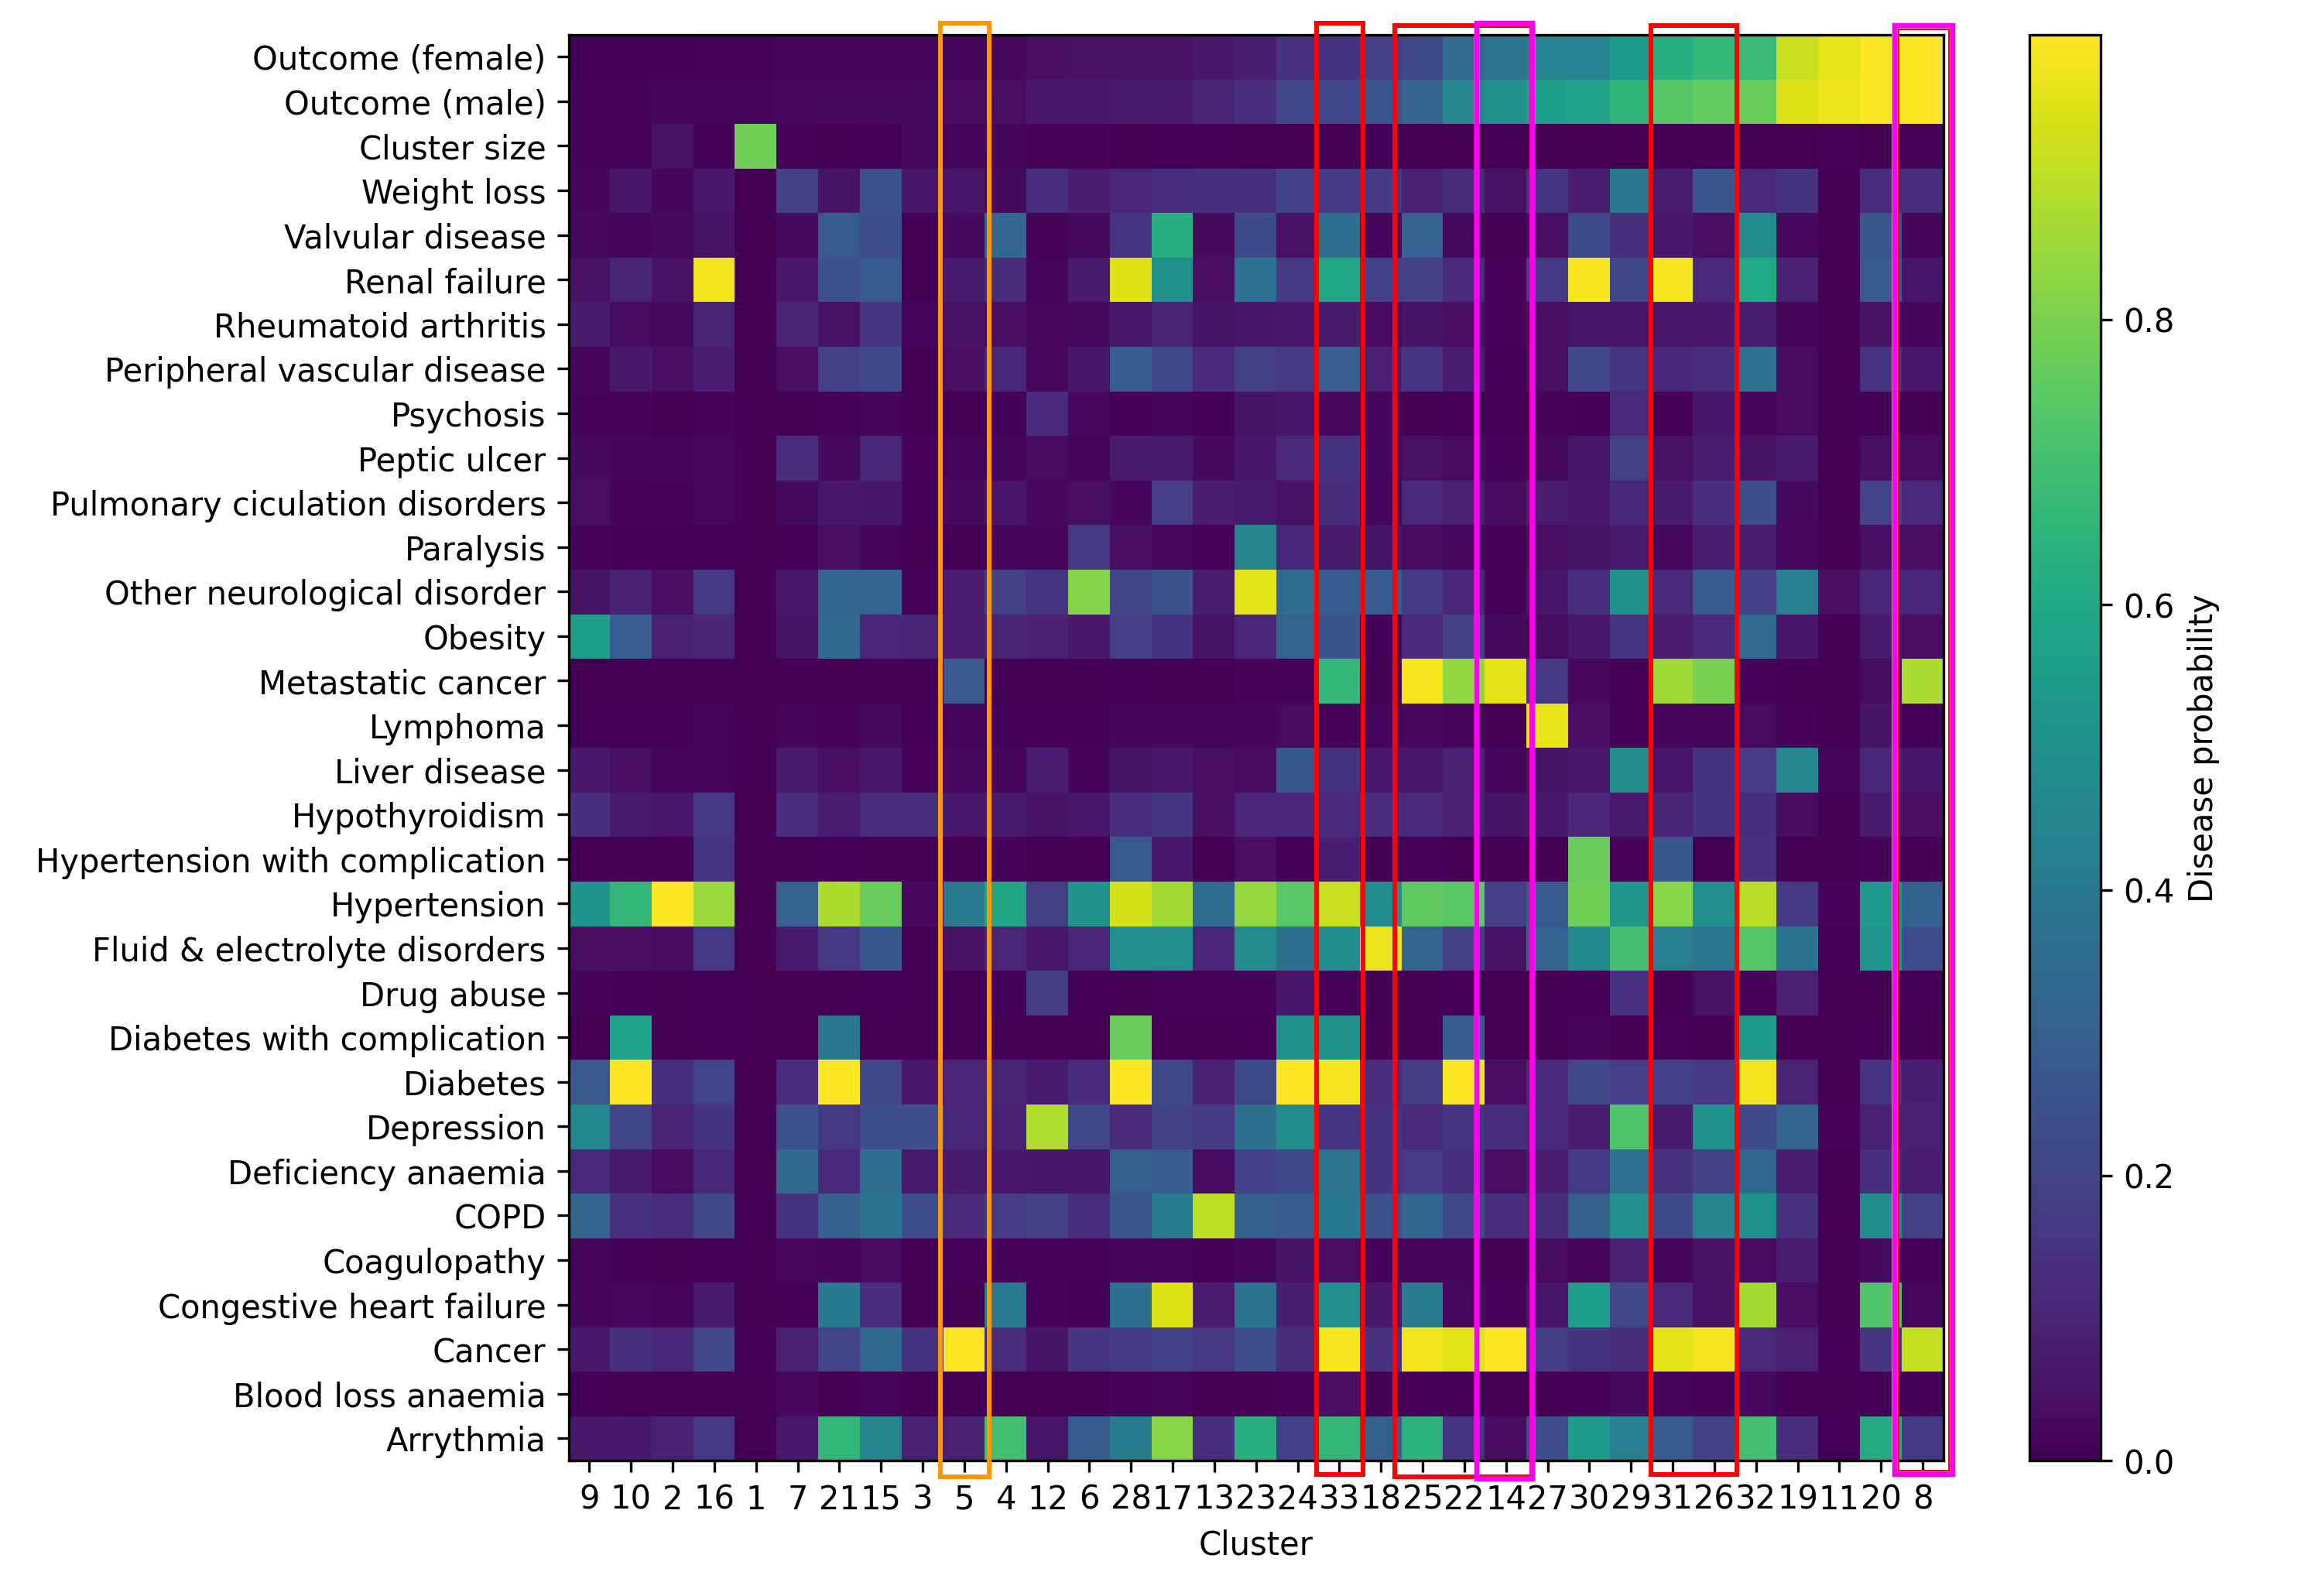
\includegraphics[width=0.8\columnwidth]{SAIL_probability_heatmap_linscale_hl.png}
\end{center}
    
\end{frame}

\begin{frame}{Summary \& Future work}
    \begin{itemize}
        \item BPR allows for granular clustering, conditioning on covariates.
        \item SVI allows Bayesian model fitting even at population-scale 
        \item Future work
        \begin{itemize}
            \item Time to event response model
            \item More exotic mixture sector structures 
        \end{itemize}
    \end{itemize}
    
\end{frame}



\begin{frame}{Thank you}
    
    Questions?
    
    \begin{center}
        \begin{tabular}{>{\centering\arraybackslash}m{4em} m{0.5\columnwidth}}
             
\includegraphics[height=1.7em]{email.png} & j.m.rafferty@swansea.ac.uk 
        \end{tabular}
    \end{center}

    \vspace{1.5em}

    {\tiny See \url{https://github.com/jim-rafferty/HDR_midlands_data_grand_rounds_20290421} for slides and notes}

    \vspace{1.5em}
    
    {\tiny
    References:
    
    \begin{itemize}

        \item[] JR et al. 2026 Bayesian Profile Regression using Variational Inference to Identify Clusters of Multiple Long-Term Conditions Conditioning on Mortality in Population-Scale Data \url{https://arxiv.org/abs/2602.24038}. Submitted to \textit{Biostatistics}

        \item[] J Molitor et al. 2010 Bayesian profile regression with an application to the National Survey of Children's Health. \textit{Biostatistics}

        \item[] S Liverani et al. 2015 PReMiuM: An R package for profile regression mixture models using Dirichlet processes. \textit{Journal of statistical software}
    
        \item[]J Lyons et al. 2021 Protocol for the development of the Wales Multimorbidity e-Cohort (WMC): data sources and methods to construct a population-based research platform to investigate multimorbidity \textit{BMJ Open}
    \end{itemize}
    }
\end{frame}

\begin{frame}[noframenumbering]{SVI - losses}

\begin{center}
    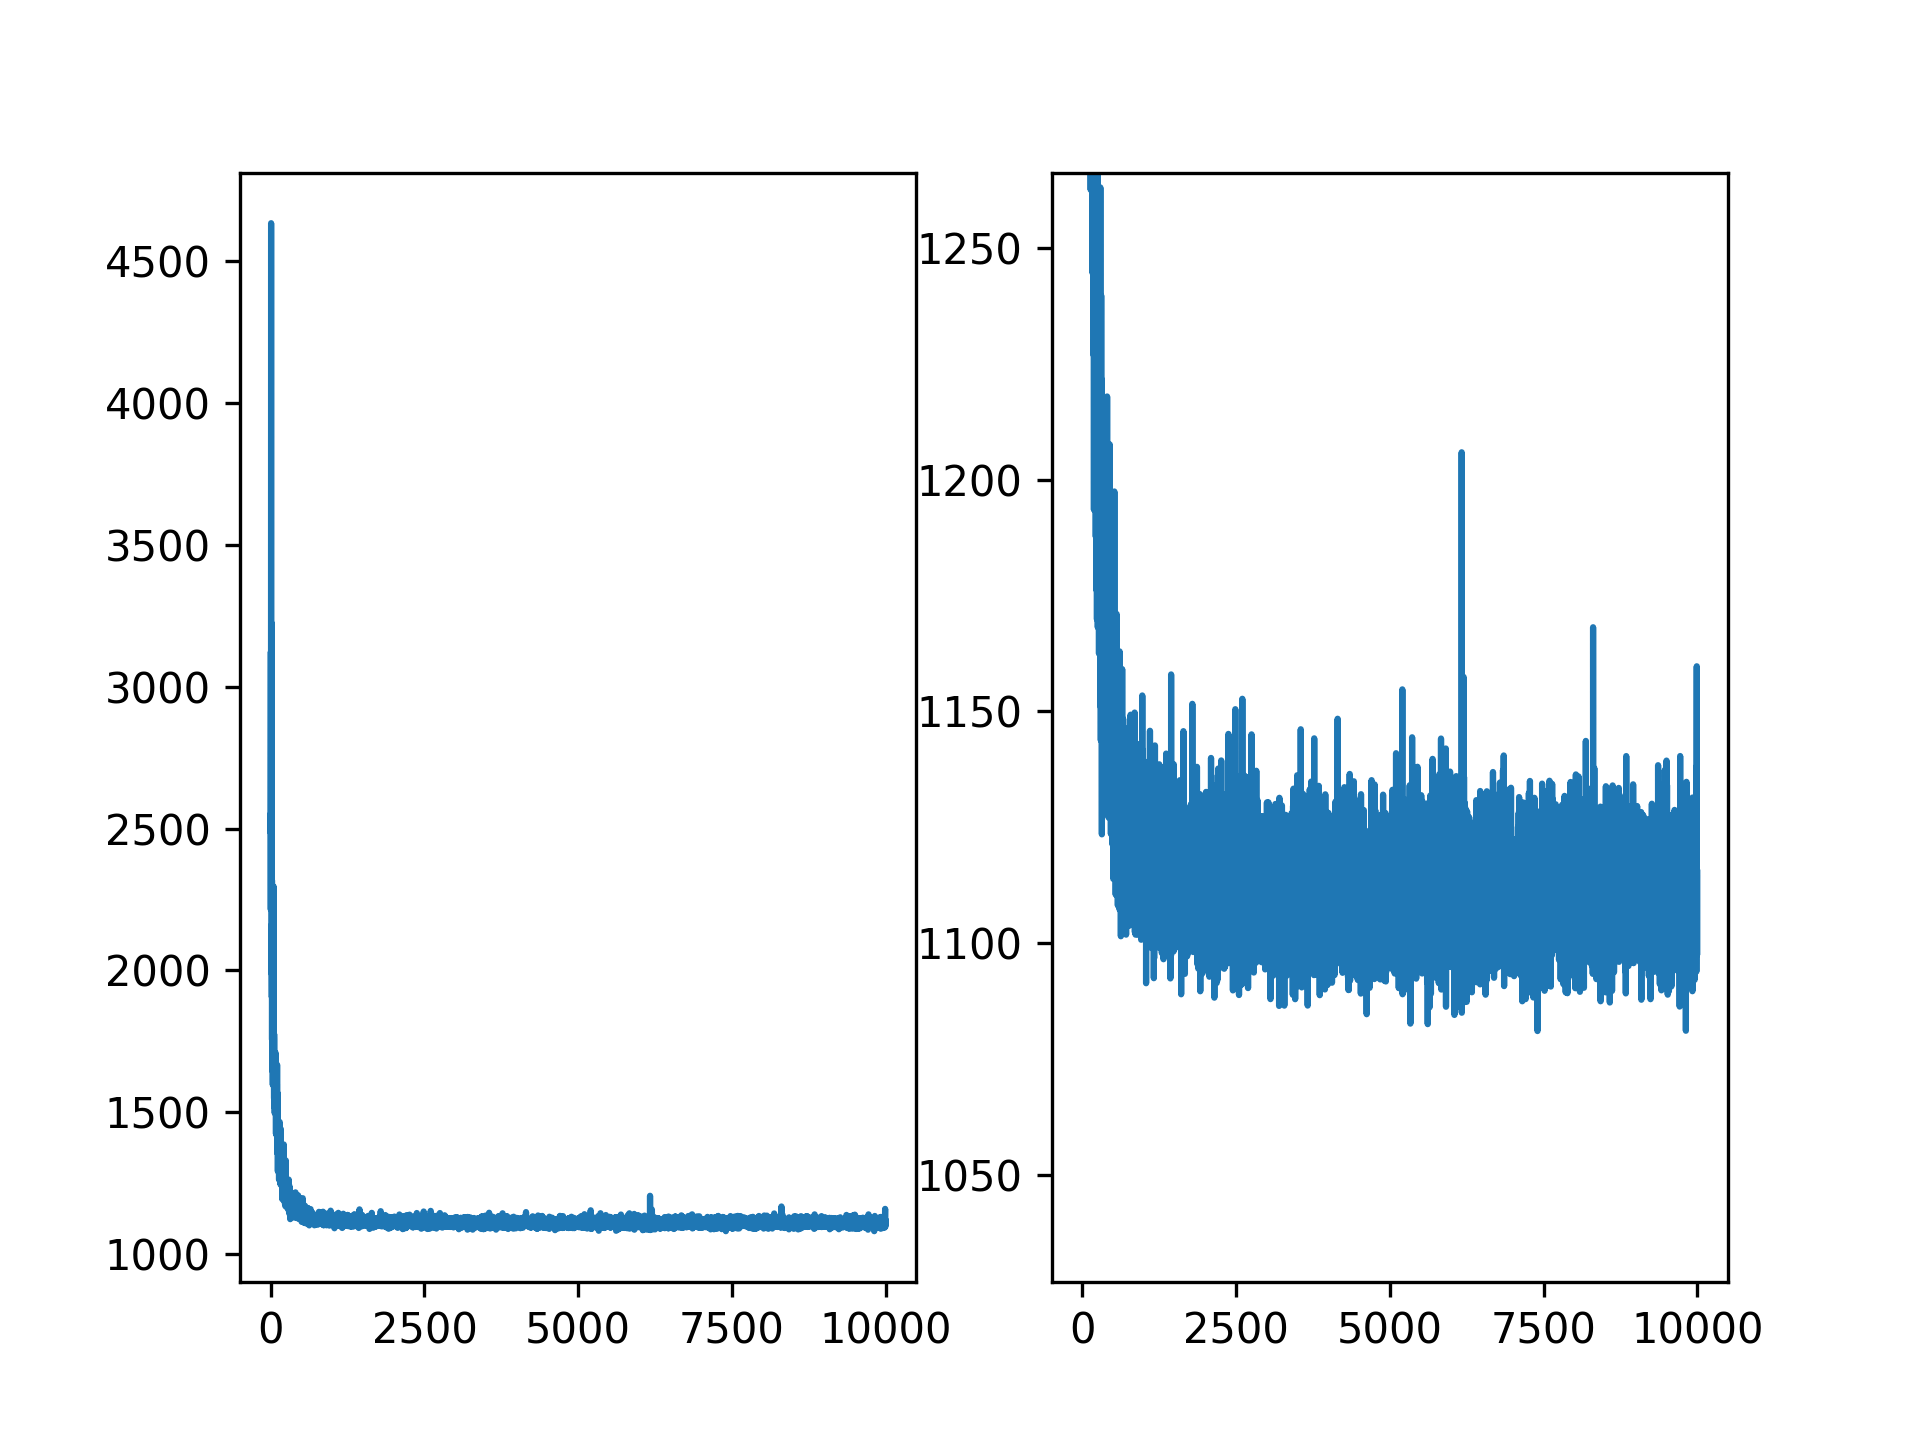
\includegraphics[width=0.7\columnwidth]{losses_ex.png}
\end{center}

\end{frame}

\end{document}
